% This is samplepaper.tex, a sample chapter demonstrating the
% LLNCS macro package for Springer Computer Science proceedings;
% Version 2.20 of 2017/10/04
%
\documentclass[runningheads]{llncs}
%
\usepackage{graphicx}
%\usepackage{amsthm}
\usepackage{amssymb}
\usepackage{mathtools}
\DeclarePairedDelimiter\abs{\lvert}{\rvert}
\DeclarePairedDelimiter\norm{\lVert}{\rVert}
\DeclarePairedDelimiter\inner{\langle}{\rangle}
\def\P{\mathcal{P}}
\DeclareMathOperator*{\argmin}{argmin}

\usepackage{algorithm}
\usepackage{algorithmic}
\makeatletter
\newcommand{\algorithmicfunction}{\textbf{function}}
\newcommand{\algorithmicendfunction}{\algorithmicend\ \algorithmicfunction}
\newenvironment{ALC@func}{\begin{ALC@g}}{\end{ALC@g}}
\newcommand{\FUNCTION}[2][default]{\ALC@it\algorithmicfunction\ #2\ %
\textbf{:}%
\ALC@com{#1}\begin{ALC@func}}
\ifthenelse{\boolean{ALC@noend}}{
    \newcommand{\ENDFUNCTION}{\end{ALC@func}}
  }{
    \newcommand{\ENDFUNCTION}{\end{ALC@func}\ALC@it\algorithmicendfunction}
  }
\makeatother

% Used for displaying a sample figure. If possible, figure files should
% be included in EPS format.
%
% If you use the hyperref package, please uncomment the following line
% to display URLs in blue roman font according to Springer's eBook style:
% \renewcommand\UrlFont{\color{blue}\rmfamily}

\begin{document}
%
\title{Info-Detection: An Information-Theoretic Approach to Detect Outlier \thanks{Supported by organization x.}}
%
%\titlerunning{Abbreviated paper title}
% If the paper title is too long for the running head, you can set
% an abbreviated paper title here
%
\author{First Author\inst{1}\orcidID{0000-1111-2222-3333} \and
Second Author\inst{2,3}\orcidID{1111-2222-3333-4444} \and
Third Author\inst{3}\orcidID{2222--3333-4444-5555}}
%
\authorrunning{F. Author et al.}
% First names are abbreviated in the running head.
% If there are more than two authors, 'et al.' is used.
%
\institute{Princeton University, Princeton NJ 08544, USA \and
Springer Heidelberg, Tiergartenstr. 17, 69121 Heidelberg, Germany
\email{lncs@springer.com}\\
\url{http://www.springer.com/gp/computer-science/lncs} \and
ABC Institute, Rupert-Karls-University Heidelberg, Heidelberg, Germany\\
\email{\{abc,lncs\}@uni-heidelberg.de}}
%
\maketitle              % typeset the header of the contribution
%
\begin{abstract}
We propose a cluster analysis-based outlier detection method called Info-Detection. The method originates from Info-clustering. We accelerate it by utilizing the hierarchical structures. The acceleration makes it possible to finish outlier detection task in reality. Info-Detection is an adaptive method and does not require any hyper parameters like outlier fraction. Experiments show that better accuracy can be achieved with an affordable time overhead.

\keywords{Outlier Detection \and Info-Clustering \and Principal Sequence of Partition.}
\end{abstract}
%
%
%
\section{Introduction}
Outlier Detection is an important task in data mining. Many algorithms such as local outlier factor, elliptic envelope and one-class SVM exist. They have some assumptions about the distribution of the data and the performance depends a lot on the hyper parameters of the method. For example, many methods require the outlier fraction as a parameter. For real-world task, it is difficult to estimate a good outlier fraction and unsuitable outlier fraction produces no good result. 

In clustering analysis, there are some adaptive methods which do not need the number of cluster as a hyper parameter. Info-clustering is such a method proposed in \cite{RN1}. It has solid theoretical foundations but is limited in application because of the algorithm complexity. In this paper, we propose a new implementation of info-clustering, which is one order of magnitude faster than the original one. This new implementation makes it possible for info-clustering to be applied on outlier detection task. 

Info-clustering is originally implemented by solving the principal sequence of partition problems for different critical values. For given critical value, a procedure called Dilworth truncation is invoked. However, different invocation of Dilworth truncation is independent and does not utilizes the intrinsic hierarchical structure of the method. By using the hierarchical tree structure, we compute latter Dilworth truncation on smaller graph. This is the basic idea of the new implementation. 

The paper is organized as follows. In section II, we make a brief introduction on info-clustering and show how it can be used to detect outlier. In Section III, we review the original algorithm of info-clustering and give our new accelerated implementation. In Section IV, we conduct experiments of outlier detection and compare Info-detection with other methods. Finally, we make the conclusion in Section V.

The notation convention of this paper is as follows: the directed graph is denoted by $G(V, E)$. Node index set $V=\{1, 2,\dots, \abs{V}\}$, node set $Z_V=\{Z_i | i \in V\}$, edge set $E=\{(i, j)\}$. Each edge is associated with a non-negative weight $w_{ij}$. $\P$ is a partition of $V$. That is, $P=\{C_1, \dots, C_k\}, \cup_{i=1}^k C_i=V$ and $i\neq j \Rightarrow C_i \cap C_j =\emptyset $. $F(\cdot)$ is the graph in-cut function, defined as $f(C)=\sum_{i \neq C, j\in C, (i,j) \in E} w_{ij}$. $\Pi$ is the collection of all partitions of $V$ and $\Pi'=\Pi\backslash\{V\}$. A partial order $ \P_1 \preceq \P_2$ on $\Pi$ is defined as
$C \in \P_1 \Rightarrow \exists C' \in \P_2 \, s.t. \, C \subseteq C'$.
Finally, $f[\cdot]$ is a function defined on $\Pi$ by $f[\P]=\sum_{C\in \P}f(C)$.

\section{Formulation of Info-Detection}
Info-detection originates from info-clustering. Info-clustering defines the cluster as follows:
\begin{equation}
C_{\gamma}(Z_V) = \textrm{maximal}\{ B \in V \vert \abs{B} > 1, I(Z_B) > \gamma \}
\end{equation}
For the given threshold $\gamma$, $C_{\gamma} (Z_V)$ represents a collection of non-intersecting subset of $V$. The shared information of $Z_B$ is defined as:
\begin{align}
I_{\P}(Z_V) & := \frac{ f[\P] }{  \abs{\mathcal{P}} - 1 }\\
I(Z_V) & := \min_{\mathcal{P} \in \Pi'(V)} I_{\mathcal{P}}(Z_V)  \label{eq:ms}
\end{align}
For sufficiently large $\gamma$, $C_{\gamma} (Z_V)$ will become empty set. The largest threshold value which makes such transition is denoted by $\gamma_N$, which has the following form:
\begin{equation}\label{eq:gammaN}
\gamma_N = \max_{B\subseteq V, \abs{B}>1} I(Z_B)
\end{equation}
In agglomerative interpretation of info-clustering \cite{RN8}, each singleton element $\{i\}$ is regarded as a leaf node of the hierarchical tree. $\gamma_N$ represents the first step to process the tree node. That is, merging elements of B to form a stem node. Traditional hierarchical clustering method using linkage criterion restricts $\abs{B}=2$. Our information criterion defined in \eqref{eq:gammaN} does not have such restriction. 

We can use $\gamma_N$ to detect anomaly in two cases. For existing nodes, suppose $\gamma_N=I(Z_B)$ and $B$ is maximal. Then nodes in $V\backslash B$  are outlier. For newly added node $i'$. Let $V'=B\cup \{i'\}$, we can compute $\gamma'_N$ for $V'$ and compare it with $\gamma_N$. If $\gamma'_N>\gamma_N$, $i'$ is normal observation since it is more integrated with existing nodes. Otherwise, $i'$ is anomaly. It can be shown that we do not need to compute $\gamma'_N$ to determine whether $\gamma'_N>\gamma_N$. We summarize our main result as follows:
\begin{proposition}\label{prop:main}
\begin{equation}
\gamma'_N > \gamma_N \iff  \sum_{i \in B} w_{ii'} > \gamma_N 
\end{equation}
\end{proposition}
From Proposition \ref{prop:main}, we can see that the computational overhead to check whether new data is normal is linear to the size of existing normal data. 
The prediction requires $\gamma_N$, whose computation is not a trivial task. It has been found that the mathematical structure of info-clustering is the same with that of principal sequence of partition(PSP) of graph. We use $\P_1, \dots, \P_k$ to denote the sequence where $\P_1 = \{V\}, \P_{i+1} \preceq \P_i$ and $\P_k = \{\{1\},\dots,\{k\}\}$.
Each $\P_i$ is the solution to the following optimization problem:
\begin{align}
h_{\P}(\lambda) &=  f[\P] - \abs{\P} \lambda  \label{eq:hPL}\\
h(\lambda) &= \min_{\P \in \Pi'(V)} h_{\P}(\lambda) \label{eq:hlambda}
\end{align}
We call $\lambda^*$ is a critical value for PSP if $\P_i, \P_{i+1}$ are both minimizer for \eqref{eq:hlambda}.
The largest critical value is equal to $\gamma_N$. However, it is difficult to solve this critical value directly without solving other critical values. The next section is focused on the algorithm to solve equation \eqref{eq:hlambda} for all $\lambda$.
\section{Improved principal sequence of partition}
The canonical way to solve equation \eqref{eq:hlambda} uses divide and conquer techniques to find the critical values and use Dilworth truncation (DT) to solve \eqref{eq:hlambda} at each specific $\lambda$ \cite{RN7}.  This implementation has $\abs{V}^2 \textrm{MF}(G)$ time complexity. \textrm{MF} represents the time complexity of maximum flow algorithm for a graph $G$. 

An improvement is proposed in \cite{RN4} using parametric maximum flow to finish the job. Although this method can achieve $\abs{V} \textrm{MF}(G)$ theoretically, it also increases the spacial complexity to $ \abs{V} \textrm{S}(G)$ where $\textrm{S}$ represents the spacial complexity to store a graph $G$. For dense graphs with $\abs{V}^2$ non-zero weight, the spacial complexity is formidable. 
% analysis of spatial complexity of pmf
Another problem of parametric maximum flow improvement is the floating point accuracy. Since this method uses the flow map of last computation to initiate the next initial flow map. The excess flow of some nodes may not be exactly zero. The non-zero excess can lead to unpredictable result and currently there is no good idea to tackle this issue. 

The above two problems prohibits such improvement from practical implementation. In this section, we abandon this approach and give another improvement which also achieves $\abs{V} \textrm{MF}(G)$ time complexity in general, only $\textrm{S}(G)$ spatial complexity and no floating point issue.

Since the PSP has the inclusion relationship, we can restrict further invocation of DT to smaller graphs. To be more specific, suppose we get $P_i = {C_1, \dots, C_t}$ for the first invocation of DT. Then we can compute PSP for each $C_i(i=1,\dots, t)$ respectively and construct those $P_j(j>i)$ from the subgraph computation. For $P_j(j<i)$, we can contract the graph $G$  to $G^t$ which has $t$ nodes by contracting each $C_i$ to a single node. By applying DT to $G^t$ can we get $P_j(j<i)$. We summarize our improved algorithm in Algorithm \ref{alg:psp_i_simplified}.

\begin{algorithm}
	\caption{An Improved Principal Sequence of Partition Algorithm}\label{alg:psp_i_simplified}
	\begin{algorithmic}[1]
		\REQUIRE a directed graph $G(V, E)$; edge cost function $c(e)$ for $e\in E$
		\ENSURE a hierarchical tree $\mathcal{T}(K, E)$ where $K \subseteq 2^{V}$ is node set and $E$ is edge set. $c'$ is edge weight map.
		\STATE initialize tree $\mathcal{T}$ with $V$ as root node, $\{j\}(j\leq \abs{V})$ as leaf node and no stem node.
		\STATE \texttt{Split}($G, V$)
		\FUNCTION{\texttt{Split}($\widetilde{G}, \widetilde{V}$)}
		\STATE $w$ is the summation of all edge weights within $\widetilde{G}$ 
		\STATE $\gamma' = \frac{w}{\abs{V(\widetilde{G})}-1}$ where $V(\widetilde{G})$ is the node set of graph $\widetilde{G}$
		\STATE $(\tilde{h}, P') = \texttt{DT}(\widetilde{G}, \gamma')$ where $\P'$ is minimizer of equation \eqref{eq:hlambda} and $\tilde{h}$ is the corresponding minimum value.  \label{alg:DT}
		\IF{$\tilde{h} = - \gamma'$}
		\STATE add edge weight $\gamma'$ in $\mathcal{T}$ starting from $\widetilde{V}$ to its children.
		\ELSE
		\FOR{$S$ in $P'$ and $\abs{S}>1$}
		\STATE make each children of $\widetilde{V}$ in $\mathcal{T}$ have new parent $S$		
		\STATE make the parent of $S$ be $\widetilde{V}$
		\STATE \texttt{Split}($\widetilde{G}[S], S$) where $\widetilde{G}[S]$ is the subgraph of $\widetilde{G}$ restricted on $S$
		\STATE contract $S$ to a single node % graph \widetilde{G} is modified
		\ENDFOR 
		\STATE \texttt{Split}($\widetilde{G}, \widetilde{V}$)		
		\ENDIF
		\ENDFUNCTION
	\end{algorithmic}
\end{algorithm}
	
\begin{figure}[!ht]
	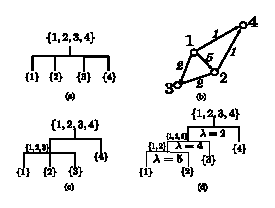
\includegraphics[width=\textwidth]{pic/alg_illustration.eps}
	\caption{Improved PSP for the graph in (b), hierarchical tree evolves from (a), (c) to (d) }\label{fig:alg_eg}
\end{figure}

\begin{example}
	We use a simple example to explain Algorithm \ref{alg:psp_i_simplified}. Consider a graph $G(V, E)$ with $V=\{1,2,3,4\}, E=\{(1,2),(1,3),(2,3),(1,4),(2,4)\}$. The weight values are $w_{13}=2, w_{12}=5, w_{23}=2, w_{14}=1, w_{24}=1$. The graph is illustrated
	in Fig. \ref{fig:alg_eg} (b). Initially, the hierarchical tree is shown in Fig. \ref{fig:alg_eg} (a). Computing $\gamma' = \frac{11}{4-1}, \tilde{h} = -\frac{16}{3} < -\gamma' $ and $\P' = \{\{1,2,3\},\{4\}\}$ from line \ref {alg:DT} in Algorithm \ref{alg:psp_i_simplified} we get the hierarchical tree shown in Fig. \ref{fig:alg_eg} (c).
	
	Then we run PSP for the subgraph $G[\{1,2,3\}]$, $\gamma' = \frac{9}{2}, \tilde{h} = -5 < -\gamma'$ and $\P= \{\{1,2\},\{3\}\}$ we get the tree shown in Fig. \ref{fig:alg_eg} (d). The other computation calculate the edge weight of $\mathcal{T}$ shown in Fig. \ref{fig:alg_eg} (d).
\end{example}		

To analyze the time complexity of Algorithm \ref{alg:psp_i_simplified}. We suppose $\abs{V} = n, \abs{E} = O(n^2)$ and highest-relabel preflow algorithm is used to solve the maximum flow problem. Then DT has $O(n^4)$ time complexity. 
We use $T(n)$ to represent the time complexity when the graph has $n$ nodes. We have the following recursive relationship. Under very general conditions, we can show that $T(n) = O(n^4)$. 

In Algorithm \ref{alg:psp_i_simplified}, the computation is done on the input graph and only has $O(n^2)$ space complexity. This is superior than parametric preflow improvement. Besides, Algorithm \ref{alg:psp_i_simplified} does not have floating accuracy problem since each DT computation is freshly started. 
\section{Experiment Result}
In this section, we first illustrate the decision boundary of info-detection by two artificial datasets. Then we conduct an experiment matrix, in which info-detection is compared with other commonly used outlier detection algorithms on both artificial and real-world datasets.

The two artificial datasets are prepared as follows:
\begin{enumerate}
\item We generate two Gaussian blobs with the same center and standard deviation 0.5. There are 255 points in total and 45 noisy points outside.
\item We generate two semi-circles which located at different centers. The 300 points on the two semi-circles are evenly distributed among all angles but deviated from the radius in Gaussian distribution. There are 45 points not belonging to the "moon" structure and are treated as outlier.
\end{enumerate}

By using the artificial dataset, we can split each into inlier set and outlier set. The boundary curve between the two sets can be used to distinuish new points. As shown by Fig. \ref{fig:boundary}, the boundary curve for info-detection is approximately the closure of the inlier figure. We also draw the decision boundary for the Elliptic Envelope method. Since this method assumes the inlier data is distributed in convex region, the decision boundary is an ellipse, which is not like the ground truth.
\begin{figure}[!ht]
	\centering
	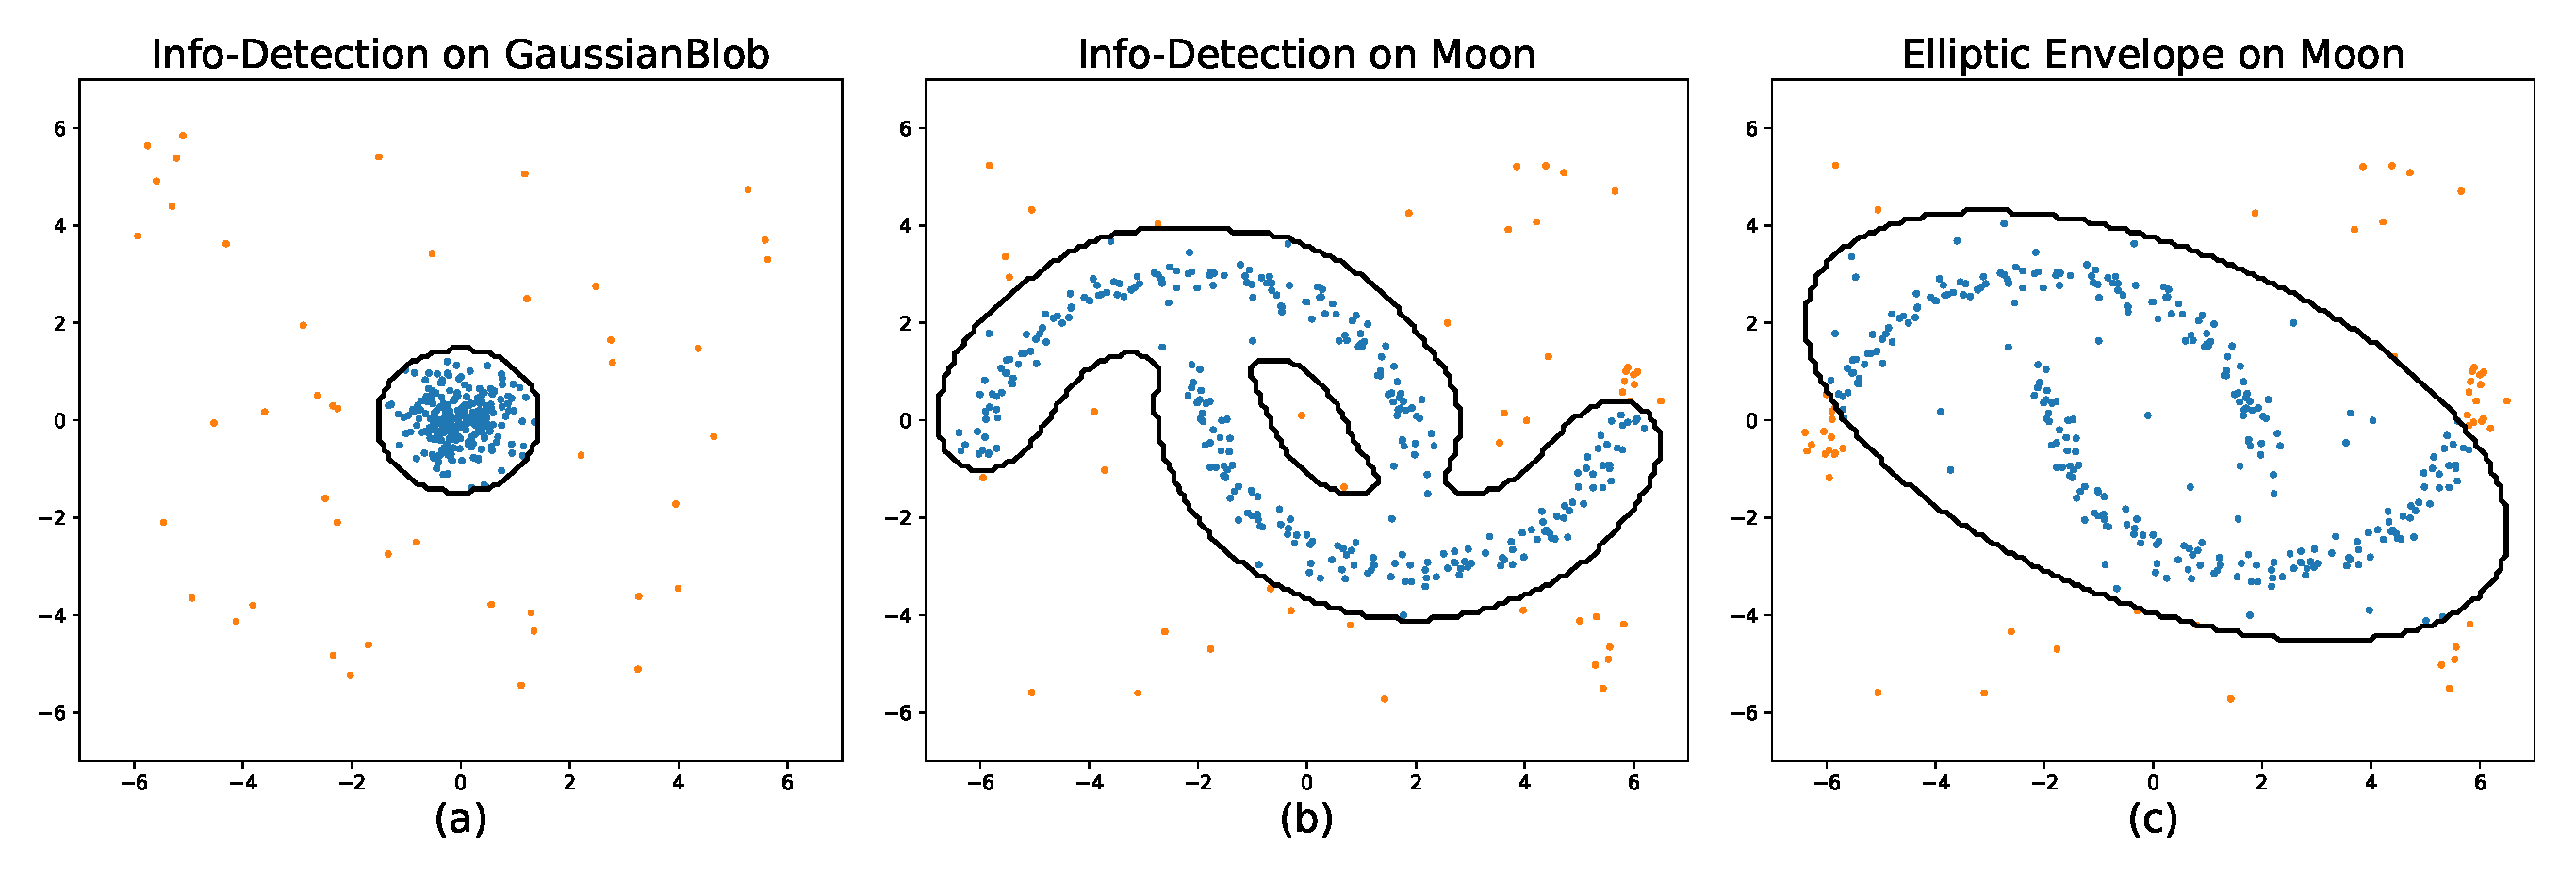
\includegraphics[width=\textwidth]{pic/outlier_boundary_illustration.eps}
	\caption{Detection boundary lines of different methods on different artificial dataset}	\label{fig:boundary}
\end{figure}

Besides the two artifical dataset, we also prepare two real-world dataset: Lymphography (first used by \cite{Lazarevic}) and Glass (\cite{hics}). Lymphography dataset has 148 instances with 6 outliers while Glass dataset has 214 instances with 7 outliers. We compare info-detection method with two commonly used method: local outlier factor detection and isolation forest. We use two metrics to measure the overall performance of the detection: true positive rate(TPR) and false negative rate(FNR). The inliner is treated as positive sample. It is difficult for a method to achieve high score on both two metrics. We manage to maximize FNR while controlling TPR $\geq 90\%$. The result is shown in Table \ref{tab:compare}.
\begin{table}[!ht]
\centering
\InputIfFileExists{../../experiment/outlier_detection/build/id_compare.tex}{}{}
\caption{Comparison of info-detection with other outlier detection algorithm on artificial and real-world dataset}\label{tab:compare}
\end{table}
%
% ---- Bibliography ----
%
% BibTeX users should specify bibliography style 'splncs04'.
% References will then be sorted and formatted in the correct style.
%
\bibliographystyle{splncs04}
\bibliography{exportlist}
%
\appendix
\section{Experiment Detail}
Since info-detection is a graph-based method, how to choose good weight between two data point is important for application of info-detection to dataset. For our experiment, several metrics are tried: 
\begin{enumerate}
\item Gaussian kernel: $w_{ij} = \exp(-\gamma \norm{x_i - x_j}^2)$
\item Laplacian kernel: $w_{ij} = \exp(-\gamma \norm{x_i - x_j}_1)$
\item kernel weight combined with k-neighbor filtering. Suppose after kernel computation and sorting we have $w_{i1} > w_{i2} > \dots > w_{in}$, then the weight assignment scheme is
$$
w'_{ij}  = 
\begin{cases}
 w_{ij} & j \leq k \\
 0 & j > k
\end{cases}
$$
This weight choice scheme has two parameters to tune: $k$ and $\gamma$. But it has two advantages. On one hand, it makes the graph have less edge and info-detection can run much faster. On the other hand, it restricts the linkage of one graph node to its k-nearest neighbors, which has more intuition in many cases.

The source code of our experiment is available \footnote{\scriptsize\url{https://github.com/zhaofeng-shu33/info-clustering-research/tree/master/experiment/outlier\_detection}} for reproducation.
For our experiment comparison, there are some additional notice.
\begin{itemize}
\item The accuracy of isolation-forest is determined by its intrinsic randomness. With the same parameter configuration, we select the result of one run of it, not possibly the best result. Info-detection and local outlier detector are deterministic method and do not have this problem.
\end{itemize}

\end{enumerate} 
\end{document}
